\documentclass[aspectratio=169]{beamer}
\usepackage{hyperref}
\usepackage[T1]{fontenc}
\usepackage{tikz}
\usepackage{xcolor}
\usepackage[french]{babel}
% A SISU beamer based on THU beamer.

% other packages
\usepackage{latexsym,amsmath,xcolor,multicol,booktabs,calligra}
\usepackage{graphicx,pstricks,listings,stackengine}
\renewcommand{\figurename}{Figure.}
\renewcommand{\tablename}{Table.}

\definecolor{appbg}{HTML}{f0f0f0}
\definecolor{chatbg}{HTML}{ffffff}
\definecolor{headerbg}{HTML}{4CAF50}
\definecolor{inputbg}{HTML}{e0e0e0}
\definecolor{sendbtn}{HTML}{4CAF50}
\definecolor{navbarbg}{HTML}{333333}
\definecolor{navbartext}{HTML}{ffffff}
\definecolor{windowborder}{HTML}{999999}

\author{Adil ABBADI}
\title{Developpement d'une Application d'Analyse de Sentiment des Commentaires sur les Media Numérique avec IA}
\institute{ENSA Agadir}
\date{\today}
\usepackage{sisu}

% defs
\def\cmd#1{\texttt{\color{red}\footnotesize $\backslash$#1}}
\def\env#1{\texttt{\color{blue}\footnotesize #1}}
\definecolor{deepblue}{rgb}{0,0,0.5}
\definecolor{deepred}{rgb}{0.6,0,0}
\definecolor{deepgreen}{rgb}{0,0.5,0}
\definecolor{halfgray}{gray}{0.55}

\lstset{
    basicstyle=\ttfamily\small,
    keywordstyle=\bfseries\color{deepblue},
    emphstyle=\ttfamily\color{deepred},    % Custom highlighting style
    stringstyle=\color{deepgreen},
    numbers=left,
    numberstyle=\small\color{halfgray},
    rulesepcolor=\color{red!20!green!20!blue!20},
    frame=shadowbox,
}


\begin{document}
\bibliographystyle{plain}
\bibliography{mybibfile}

\begin{frame}

    \begin{figure}[H]
        \begin{center}
            
\includegraphics[width=0.3\linewidth]{assets/images/logo.png}
            \hfill
            
\includegraphics[width=0.3\linewidth]{assets/images/code.png}
        \end{center}
    \end{figure}

    \titlepage



    \begin{tikzpicture}[remember picture, overlay]
        % Define the coordinates where you want the block to be placed
        \coordinate (block) at ([yshift=-8.3cm]current page.north);

        % Place the block at the defined coordinates
        \node[above, text width=\linewidth, text=black,fill = white] at (block) {
            \begin{minipage}{\linewidth}
                \centering
                \begin{minipage}[t]{0.45\linewidth}
                    \begin{center}
                        \small
                        \textbf{Jury:} \\
                        M. A EL YOUSFI \\
                        M. H AKSASSE \\
                        M. M ELYAAKOUBI \\



                        % Ajoutez d'autres membres du jury si nécessaire
                    \end{center}
                \end{minipage}
                \hfill
                \begin{minipage}[t]{0.45\linewidth}
                    \begin{center}
                        \small
                        \textbf{Encadré par:} \\
                        M. A EL YOUSFI\\
                        M. H Elkina\\


                        % Ajoutez d'autres encadrants si nécessaire
                    \end{center}
                \end{minipage}
            \end{minipage}
        };
    \end{tikzpicture}

\end{frame}


\begin{frame}
    \tableofcontents[sectionstyle=show,subsectionstyle=show/shaded/hide,subsubsectionstyle=show/shaded/hide]
\end{frame}

\section{Introduction}

\subsection{Contexte general}

\begin{frame}{Organisme d'accueil}

    \vspace{0.5cm} % Adjust space between image and text
    \begin{block}{\centering \textbf{\Large Le centre Code 212}}
        \centering
        \vspace{0.2cm} % Adjust space within the block
        Code 212 : Hub d'excellence numérique du PACTE ESRI-2030. Centre de compétences spécialisé en transformation digitale, offrant certification professionnelle et solutions innovantes alignées sur les exigences du marché.
    \end{block}

    \begin{figure}[H]
        \centering
        \begin{minipage}[b]{0.45\linewidth}
            \centering
            
            
\includegraphics[width=\linewidth]{assets/images/esri.png}
        \end{minipage}
        \begin{minipage}[b]{0.45\linewidth}
            \centering
            
\includegraphics[width=\linewidth]{assets/images/code.png}
        \end{minipage}
    \end{figure}
\end{frame}


\begin{frame}{Centre Code212 : Ses Fonctionnalités et Services}

    \begin{figure}[H]
        \centering
        \begin{minipage}[b]{0.45\linewidth}
            \centering
            
\includegraphics[width=\linewidth]{assets/images/formation.jpg}
        \end{minipage}
        \begin{minipage}[b]{0.45\linewidth}
            \centering
            
\includegraphics[width=\linewidth]{assets/images/certificat.png}
        \end{minipage}
    \end{figure}
\end{frame}



\subsection{Problématique}
\begin{frame}{Problématique}
    \begin{figure}[H]
        \centering
        
\includegraphics[height=3cm]{assets/images/question.png}
    \end{figure}
    
    \vspace{0.5cm}
    
    \begin{block}{\centering \textbf{Défis de l'Analyse de Sentiments}}
        \begin{itemize}
            \setlength\itemsep{0.6em}
            \item \textbf{Volume de données} : Milliers de commentaires quotidiens sur Hespress
            \item \textbf{Analyse manuelle} : Processus chronophage et subjectif
            \item \textbf{Temps réel} : Besoin d'analyse instantanée des sentiments
        \end{itemize}
    \end{block}
    
    \vspace{0.3cm}
    
    \begin{alertblock}{\centering \textbf{Problématique}}
        \centering
        Comment analyser efficacement les sentiments exprimés dans les commentaires des actualités Hespress pour comprendre l'opinion publique marocaine en temps réel ?
    \end{alertblock}
\end{frame}

\subsection{Solution proposee}
\begin{frame}{Solution proposee}
    Application de classification de sentiments des commentaires Hespress : analyse automatisée en temps réel de l'opinion publique via intelligence artificielle et architecture microservices moderne.
    \begin{figure}[H]
        \centering
        
\includegraphics[height=3cm]{assets/images/ia.png}
    \end{figure}
\end{frame}

\begin{frame}{Architecture Technique}
    \begin{block}{\centering \textbf{Stack Technologique}}
        \begin{itemize}
            \setlength\itemsep{0.6em}
            \item \textbf{Frontend} : Next.js pour une interface moderne
            \item \textbf{Backend} : FastAPI pour des API performantes
            \item \textbf{Base de données} : PostgreSQL avec cache Redis
            \item \textbf{Authentification} : Keycloak pour la sécurité
            \item \textbf{Scraping} : Selenium pour l'extraction de données
            \item \textbf{IA} : Modèle cardiffnlp/twitter-xlm-roberta-base-sentiment
            \item \textbf{API Gateway} : Spring pour l'orchestration
        \end{itemize}
    \end{block}
\end{frame}

\subsection{Fonctionnalités attendues}

\begin{frame}{Fonctionnalités Axées sur l'Utilisateur}
    \begin{figure}[H]
        \centering
        
\includegraphics[height=3cm]{assets/images/user.png}
    \end{figure}
    \begin{itemize}
        \setlength\itemsep{0.8em} % Adjust the spacing between items
        \item \textbf{Visualisation des sentiments en temps réel}
        \item \textbf{Recherche et filtrage par article}
        \item \textbf{Statistiques et graphiques d'analyse}
        \item \textbf{Export des données d'analyse}
    \end{itemize}
\end{frame}

\begin{frame}{Fonctionnalités Axées sur l'administrateur}
    \begin{figure}[H]
        \centering
        
\includegraphics[height=3cm]{assets/images/admin.png}
    \end{figure}

    \begin{itemize}
        \setlength\itemsep{0.8em} % Adjust the spacing between items
        \item \textbf{Configuration du scraping Hespress}
        \item \textbf{Monitoring système et performances}
        \item \textbf{Gestion des utilisateurs et permissions}
        \item \textbf{Gestion des logs et alertes}
    \end{itemize}
\end{frame}

\section{Analyse et Conception du Project}
\subsection{Analyse du besoin}
\begin{frame}{Analyse du besoin}
    \begin{figure}[H]
        \centering
        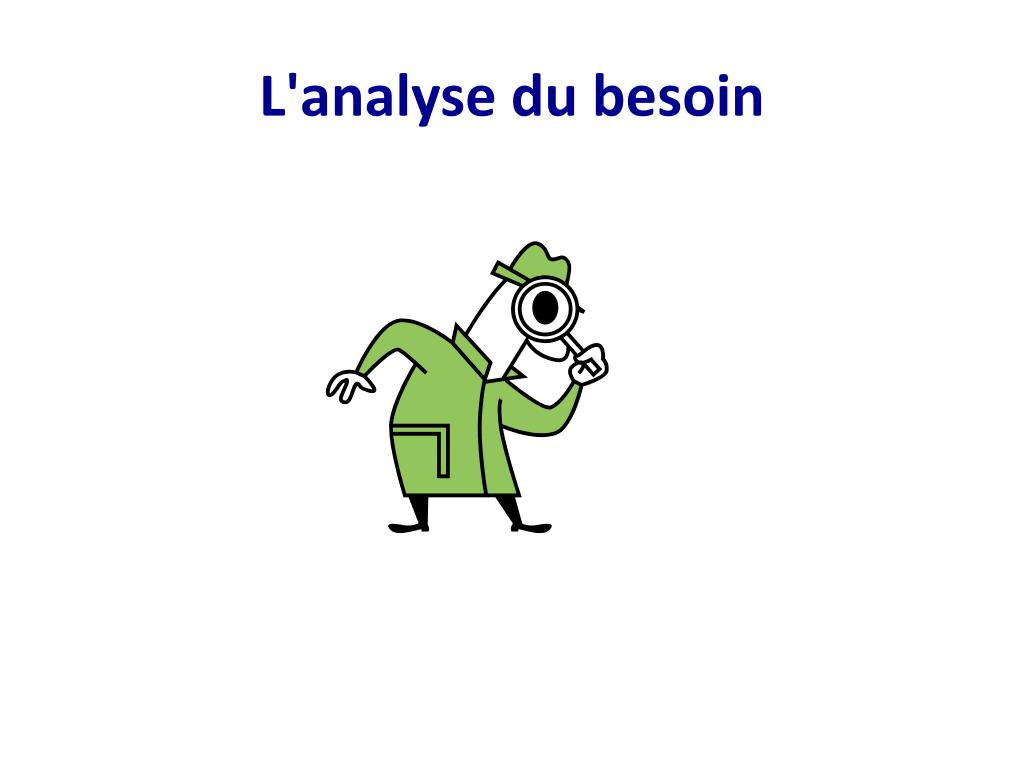
\includegraphics[height=5cm]{assets/images/analyse-besoin.jpg}
    \end{figure}

\end{frame}

\subsection{Digramme cas d'utilisation}
\begin{frame}{Digramme cas d'utilisation}
    \begin{figure}[H]
        \centering
        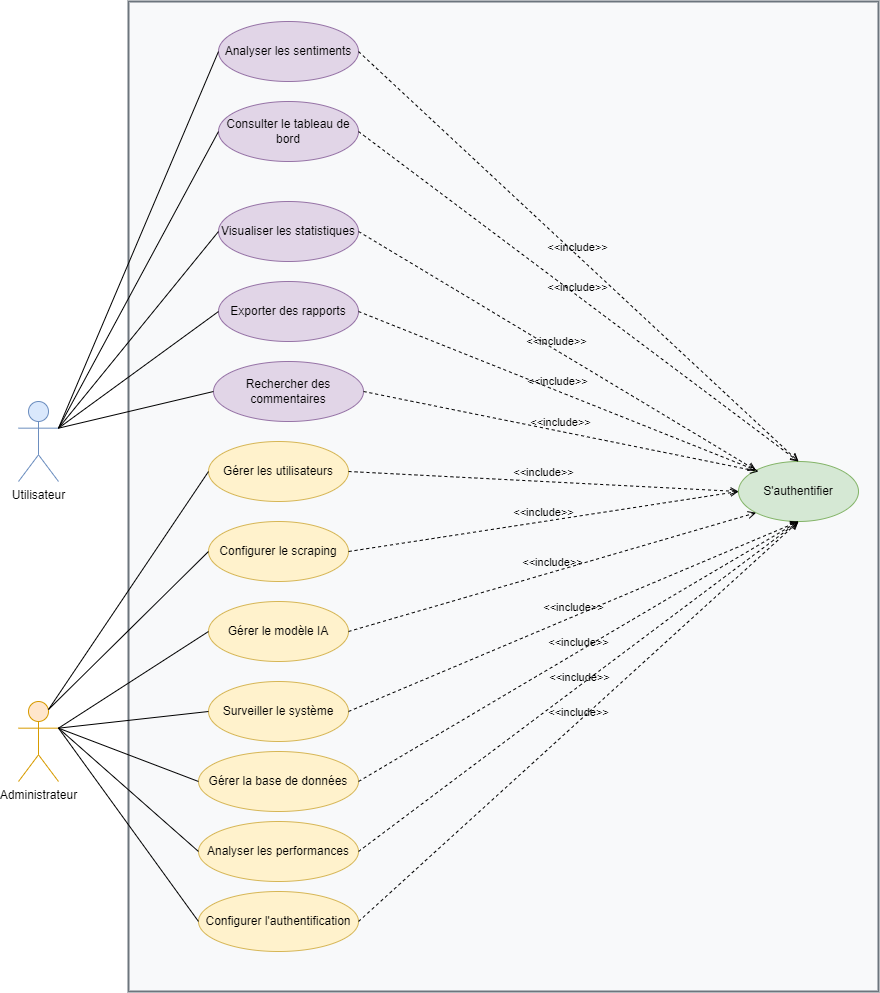
\includegraphics[scale=0.2]{assets/images/usecase.png}
    \end{figure}
\end{frame}


\subsection{Architecture microsevice}

\begin{frame}{Architecture microservice}
    \begin{figure}[H]
        \centering
        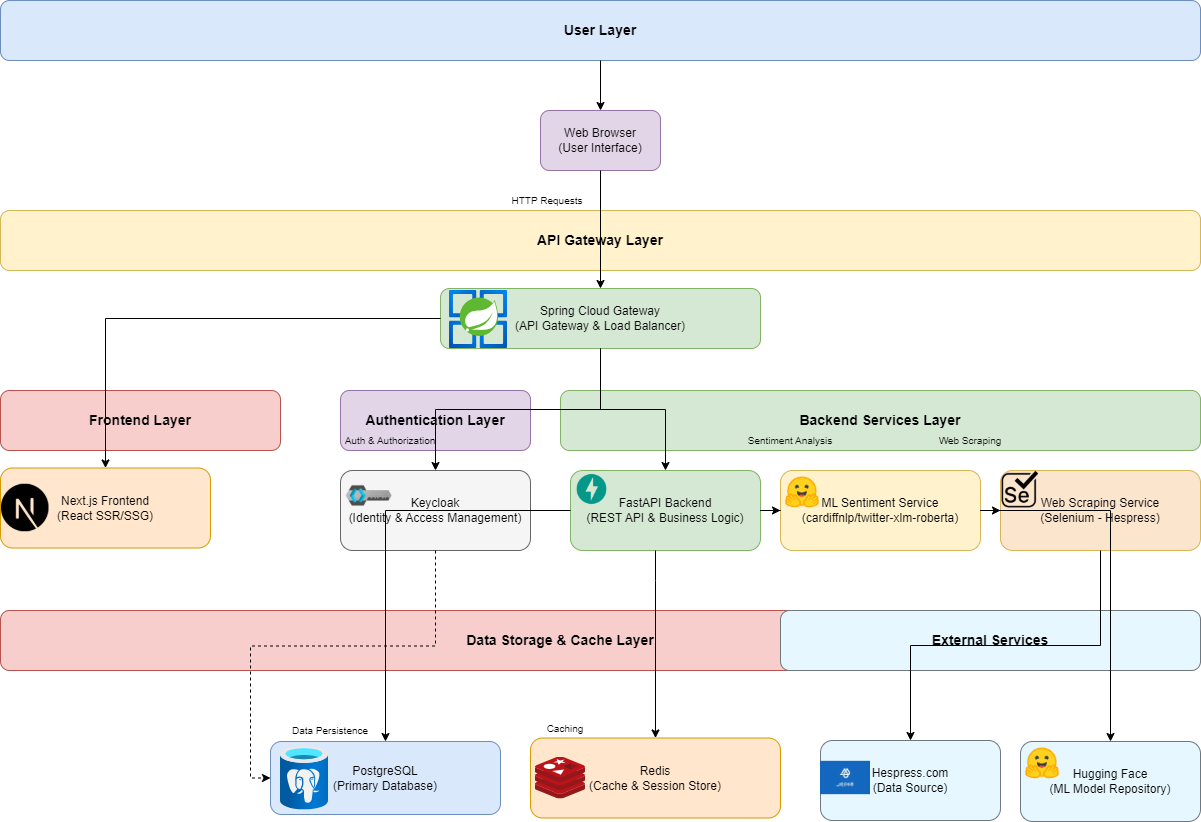
\includegraphics[height=6cm]{assets/images/arch.png}
    \end{figure}
\end{frame}




\subsection{Methodology}
\begin{frame}{Methodology}

    \begin{figure}[H]
        \centering
        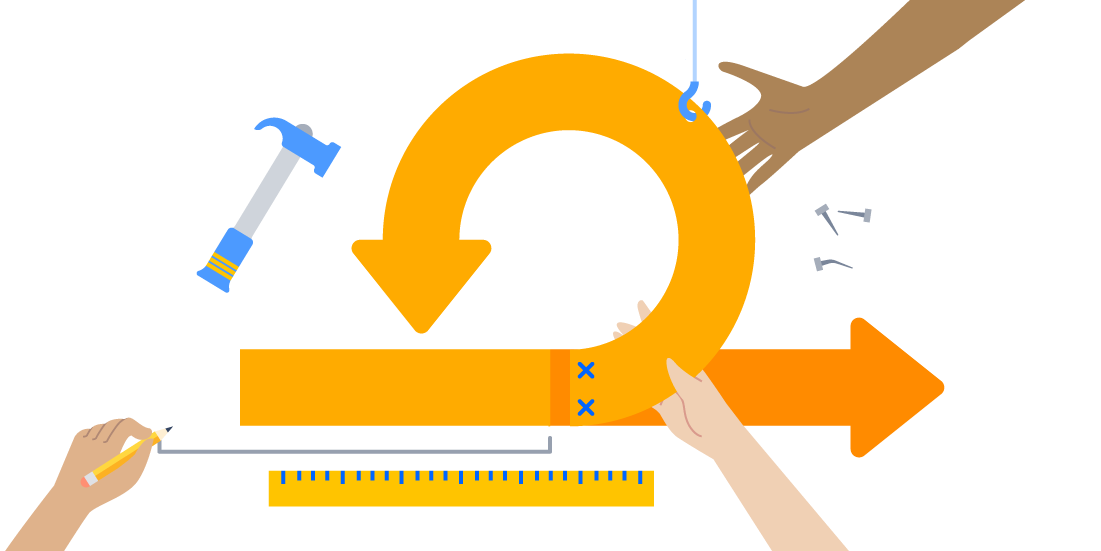
\includegraphics[height=4cm]{assets/images/scrum.png}
    \end{figure}

    Afin de gérer au mieux ce projet, nous avons opté pour la méthode SCRUM et divisé les différents modules en sprints.
\end{frame}


\subsection{Planification}
\begin{frame}{Planification}

    \begin{figure}[H]
        \centering
        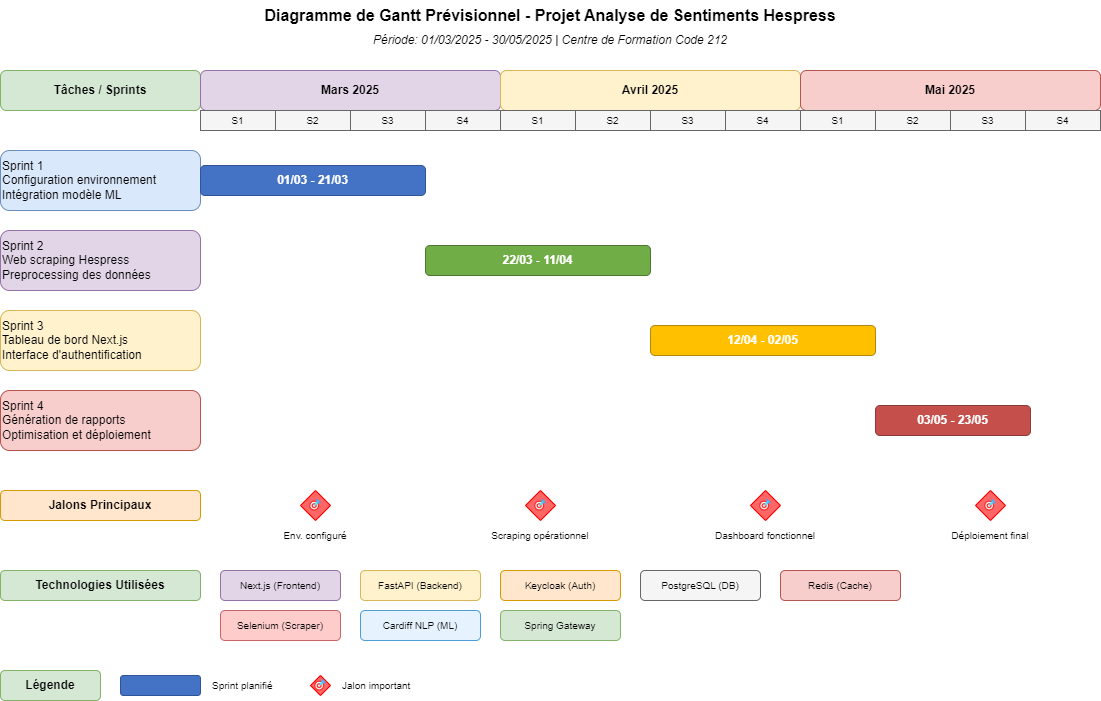
\includegraphics[scale=0.3]{assets/images/gantt-previsionnel.png}
    \end{figure}
\end{frame}






\section{Spécifications Techniques}


\subsection{Évaluation comparative des technologies.}
\begin{frame}{Benchmark Backend}
    \begin{figure}[htpb]
        \centering
        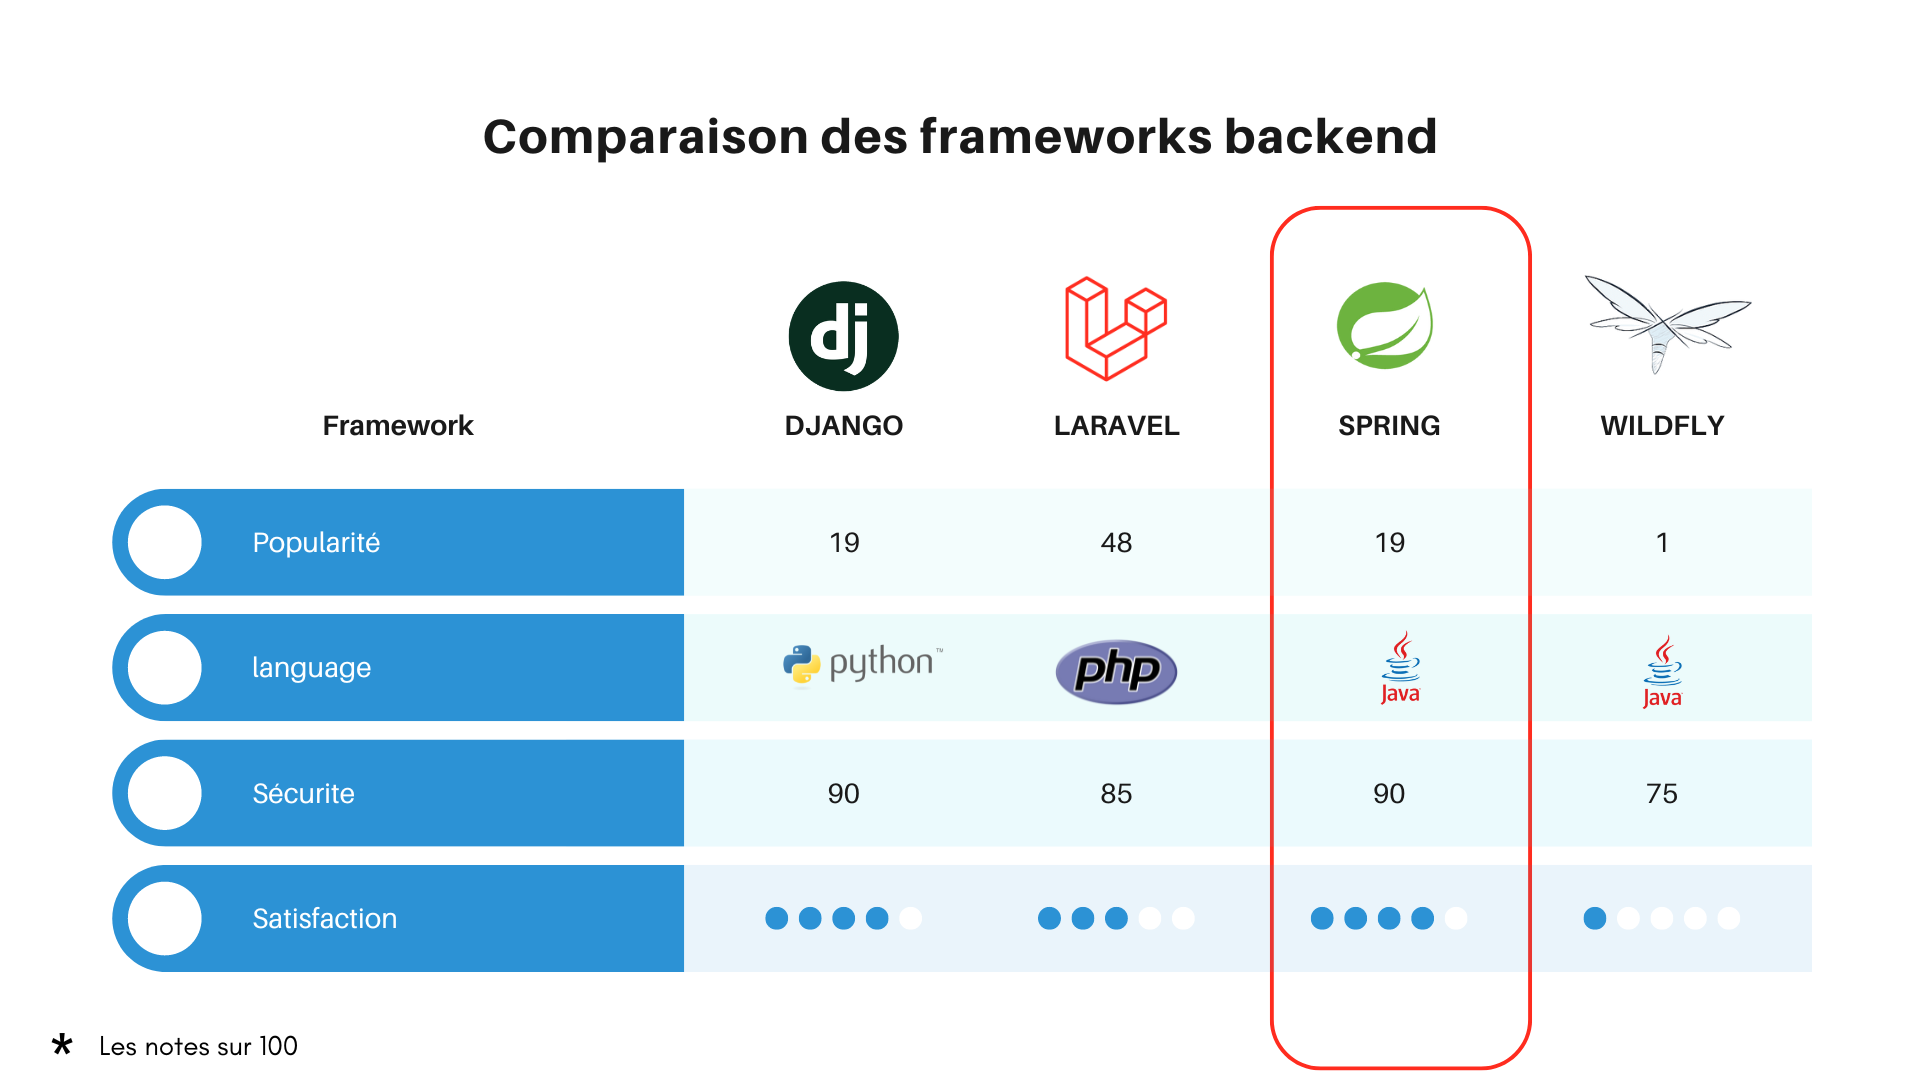
\includegraphics[height=5cm]{assets/images/benchmark.png}
    \end{figure}
\end{frame}

\begin{frame}{Benchmark Fronted}
    \begin{figure}[htpb]
        \centering
        
\includegraphics[height=5cm]{assets/images/bench-next.jpg}
    \end{figure}
\end{frame}

\begin{frame}{Benchmark model IA}
    \begin{figure}[htpb]
        \centering
        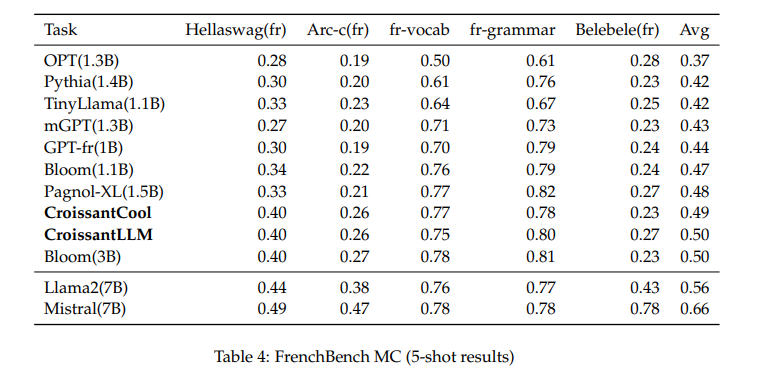
\includegraphics[height=6cm]{assets/images/ia_benchmark.png}
    \end{figure}
\end{frame}

\subsection{Technologies Sélectionnées}
\begin{frame}{Technologies choisies pour les services}
    \begin{figure}[htpb]
        \centering
        \begin{minipage}{0.32\textwidth}
            \centering
            
\includegraphics[height=3cm]{assets/images/next.png}
        \end{minipage}%
        \hspace{0.03\textwidth}
        \begin{minipage}{0.32\textwidth}
            \centering
            
\includegraphics[height=3cm]{assets/images/spring.png}
        \end{minipage}%
        \hspace{0.03\textwidth}
        \begin{minipage}{0.32\textwidth}
            \centering
            
\includegraphics[height=3cm]{assets/images/keycloak.png}
        \end{minipage}

    \end{figure}
\end{frame}



\begin{frame}{Technologies choisies pour IA}
    \begin{figure}[htpb]
        \centering

        \begin{minipage}{0.5\textwidth}
            \centering
            
\includegraphics[height=2cm]{assets/images/tinyllama.png}
        \end{minipage}
        \hspace{0.1\textwidth}
        \begin{minipage}{0.5\textwidth}
            \centering
            
\includegraphics[height=2cm]{assets/images/langchain.jpeg}
        \end{minipage}
        \hspace{0.1\textwidth}
        \begin{minipage}{0.5\textwidth}
            \centering
            
\includegraphics[height=2cm]{assets/images/mongo.png}
        \end{minipage}
    \end{figure}
\end{frame}

\subsection{Communication entre services}
\begin{frame}{Communication entre services}
    \begin{figure}[htpb]
        \centering
        
\includegraphics[height=2cm]{assets/images/rest.png}
        \hspace{0.1\textwidth}
        
\includegraphics[height=2cm]{assets/images/kafka.png}
    \end{figure}
\end{frame}

\subsection{Conclusion}
\begin{frame}{Conclusion}

    Cette étude technique détaille l\'architecture des microservices, les technologies utilisées, et les interactions entre les services, garantissant une application modulaire, sécurisée, et scalable avec Keycloak pour la gestion des identités et des accès. Les choix de conception visent à assurer une expérience utilisateur optimale tout en garantissant performance et sécurité.
\end{frame}

\section{Realisation et mise en oeuvre}
\subsection{Sprint 1: D´eveloppement et D´eploiement du Chatbot}
\begin{frame}{Diagramme de cas d'utilisation}

    \begin{figure}[htpb]
        \centering
        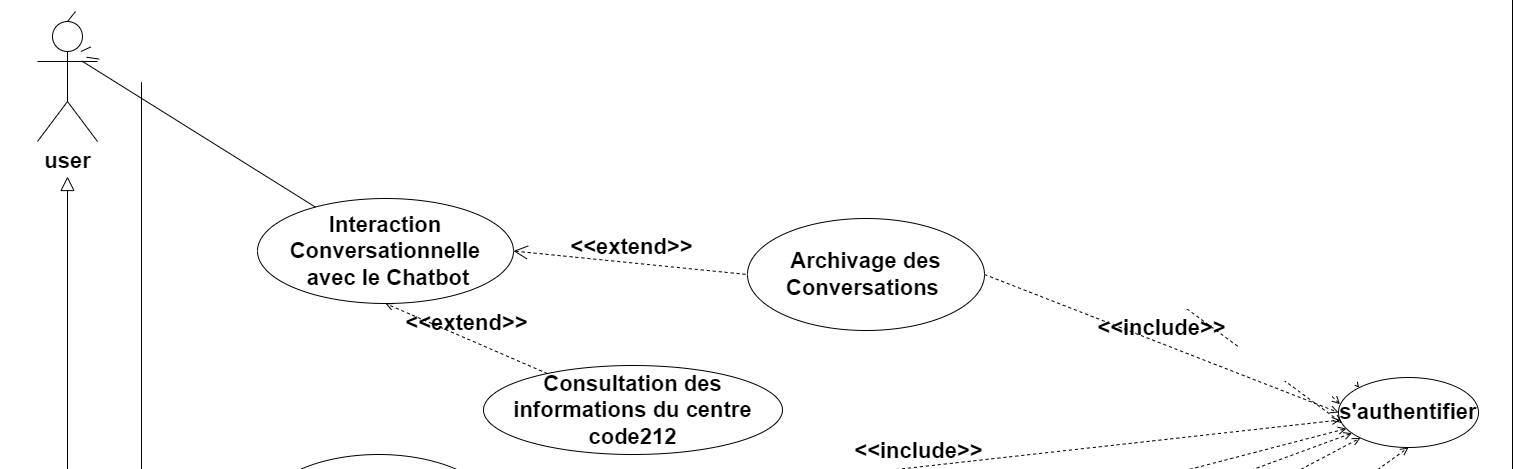
\includegraphics[height=4cm]{assets/images/sprint1-usecase.png}
    \end{figure}
\end{frame}

\begin{frame}{Diagramme de classe}

    \begin{figure}[htpb]
        \centering
        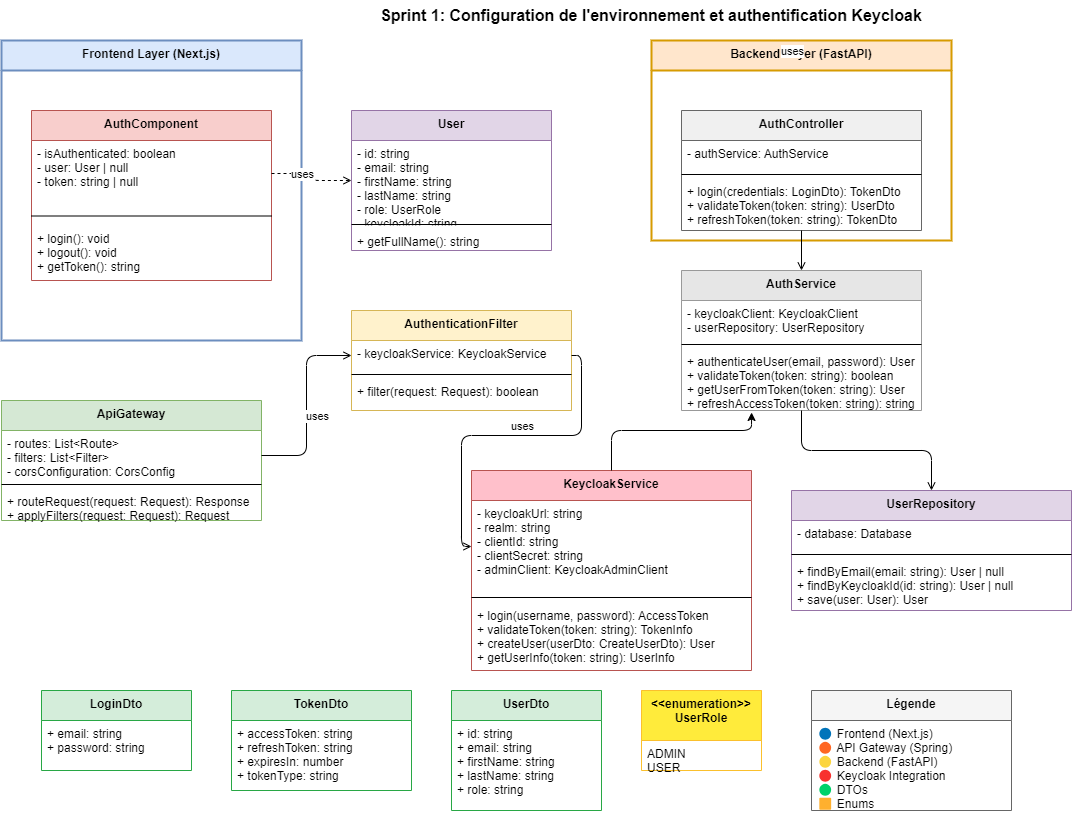
\includegraphics[height=5cm]{assets/images/sprint1-class.png}
    \end{figure}
\end{frame}

\begin{frame}{Diagramme de sequence}
    \begin{figure}[htpb]
        \centering
        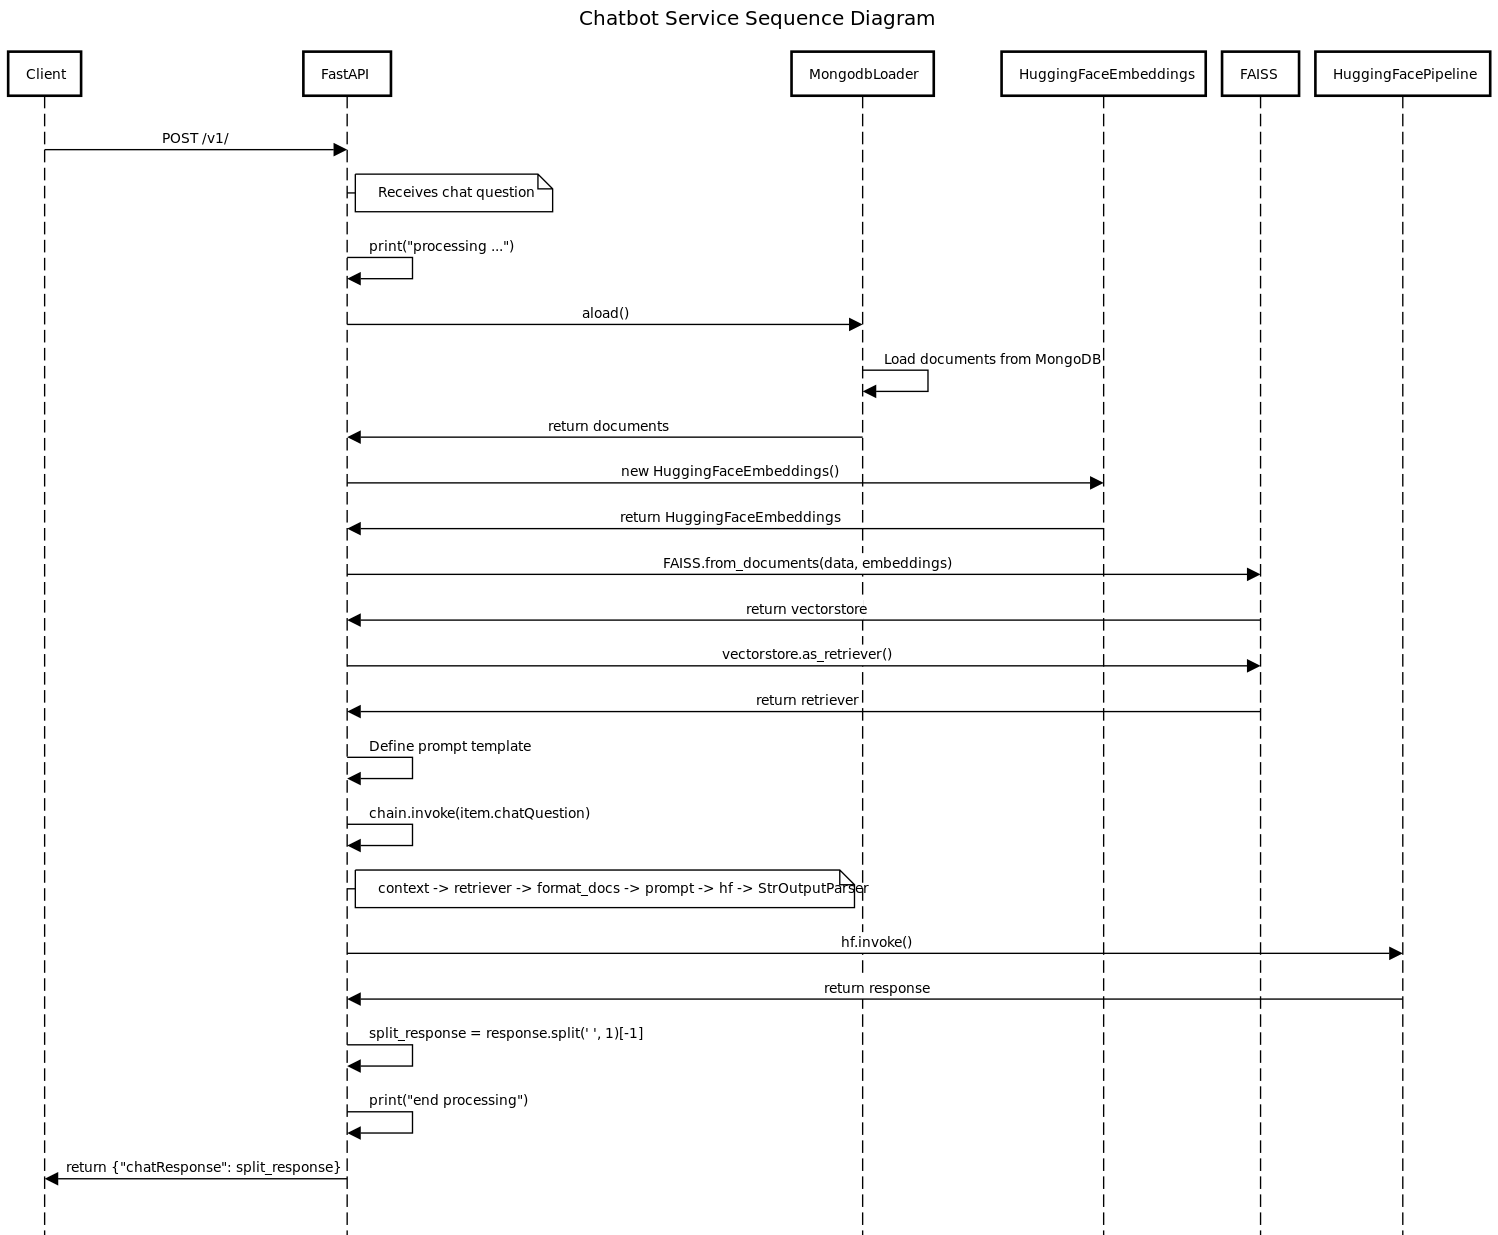
\includegraphics[height=8cm]{assets/images/chatbot-seq.png}
    \end{figure}
\end{frame}

\begin{frame}{Realisation}
    \begin{figure}[htpb]
        \centering
        
\includegraphics[height=6cm]{assets/images/chat2.png}
    \end{figure}
\end{frame}


\subsection{Sprint 2: Authentification et mise a jour de la
    base de donnees par l’administrateur}
\begin{frame}{Diagramme de cas d'utilisation}

    \begin{figure}[htpb]
        \centering
        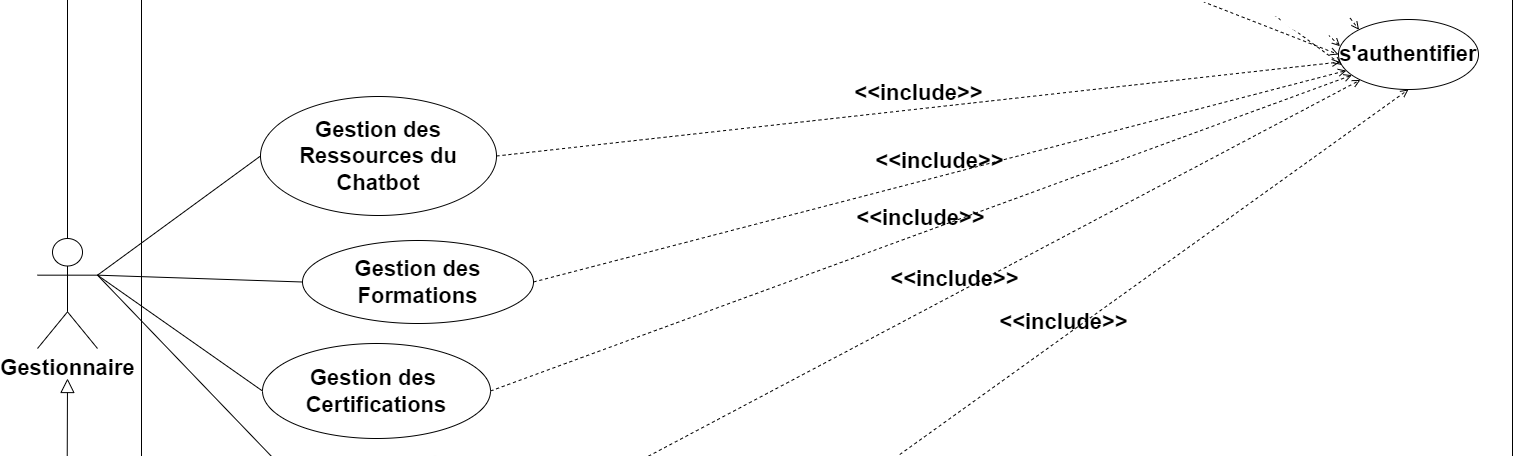
\includegraphics[height=4cm]{assets/images/sprint2-usecase.png}
    \end{figure}
\end{frame}

\begin{frame}{Diagramme de classe}

    \begin{figure}[htpb]
        \centering
        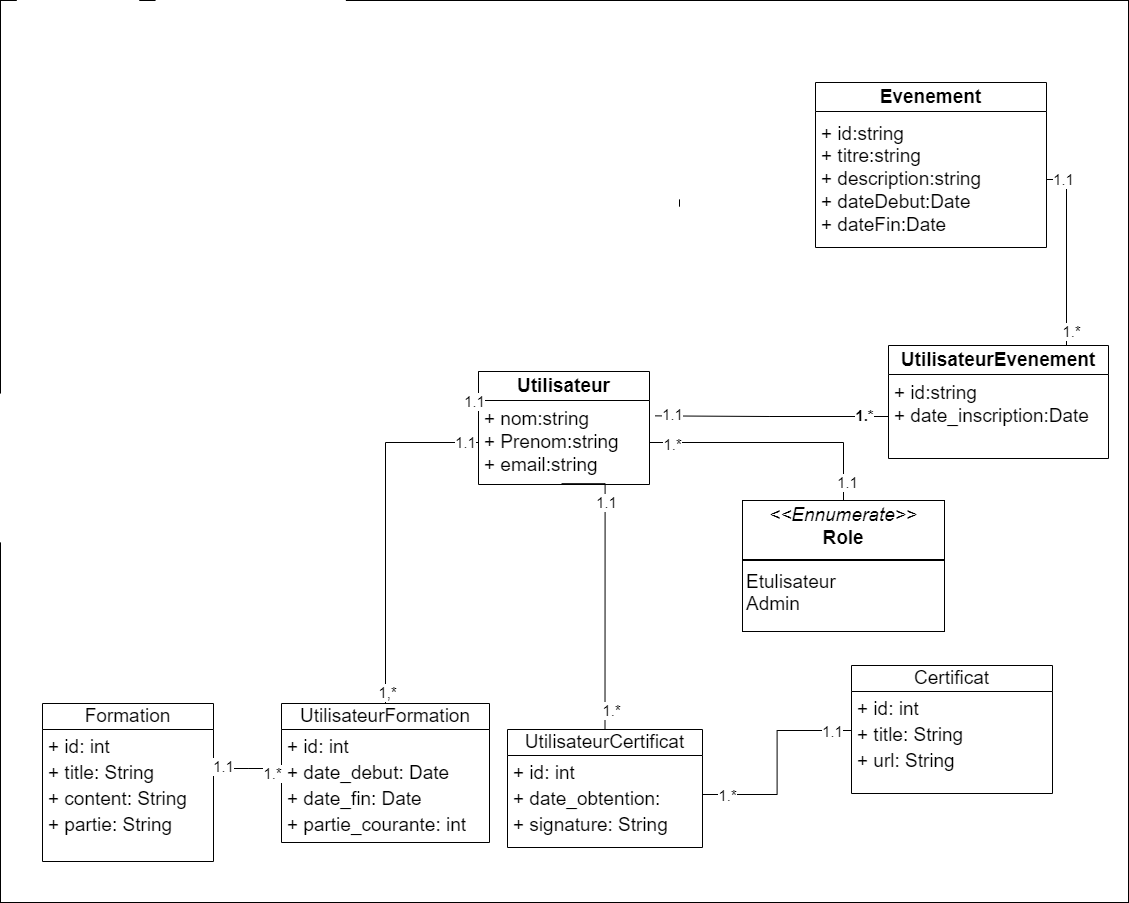
\includegraphics[height=5cm]{assets/images/sprint2-class.png}
    \end{figure}
\end{frame}

\begin{frame}{Diagramme de sequence d'authentification}
    \begin{figure}[htpb]
        \centering
        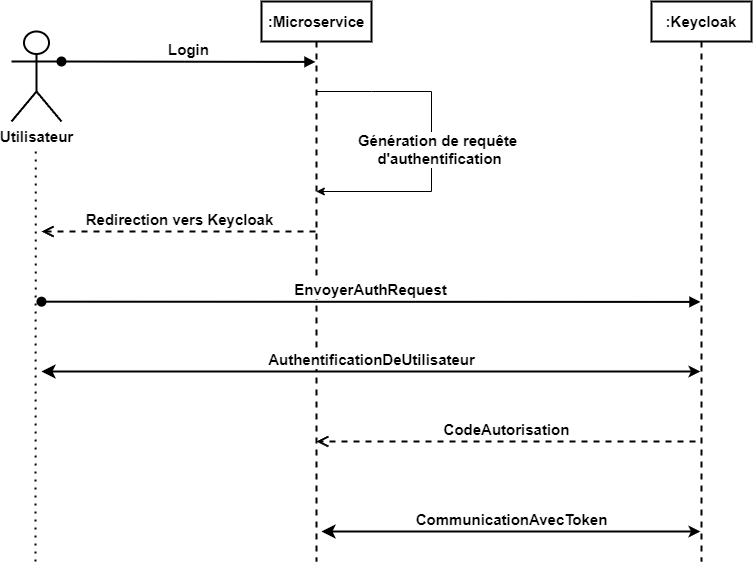
\includegraphics[height=8cm]{assets/images/keycloak-seq.png}
    \end{figure}
\end{frame}

\begin{frame}{Diagramme de sequence de gestion des resources du chatbot}
    \begin{figure}[htpb]
        \centering
        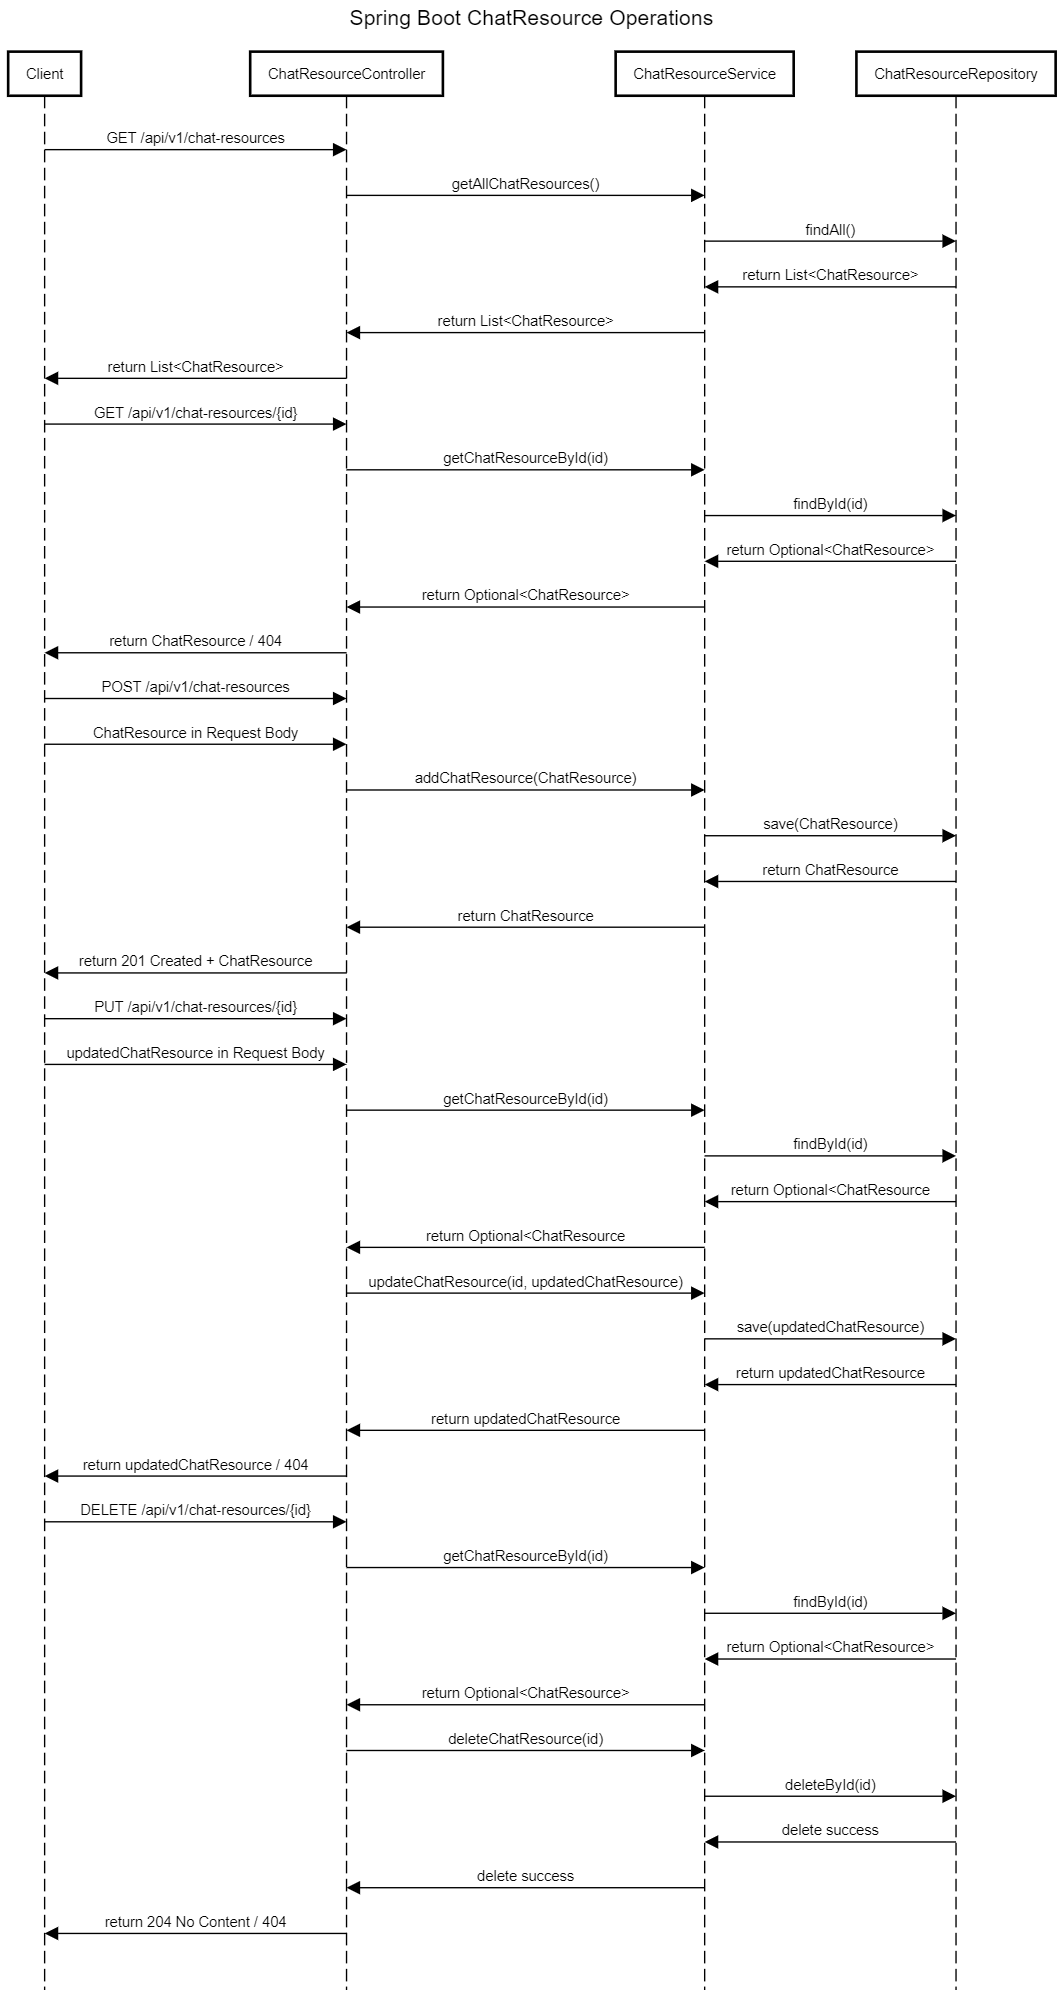
\includegraphics[height=8cm]{assets/images/chat-res-seq.png}
    \end{figure}
\end{frame}

\begin{frame}{Realisation}
    \begin{figure}[htpb]
        \centering
        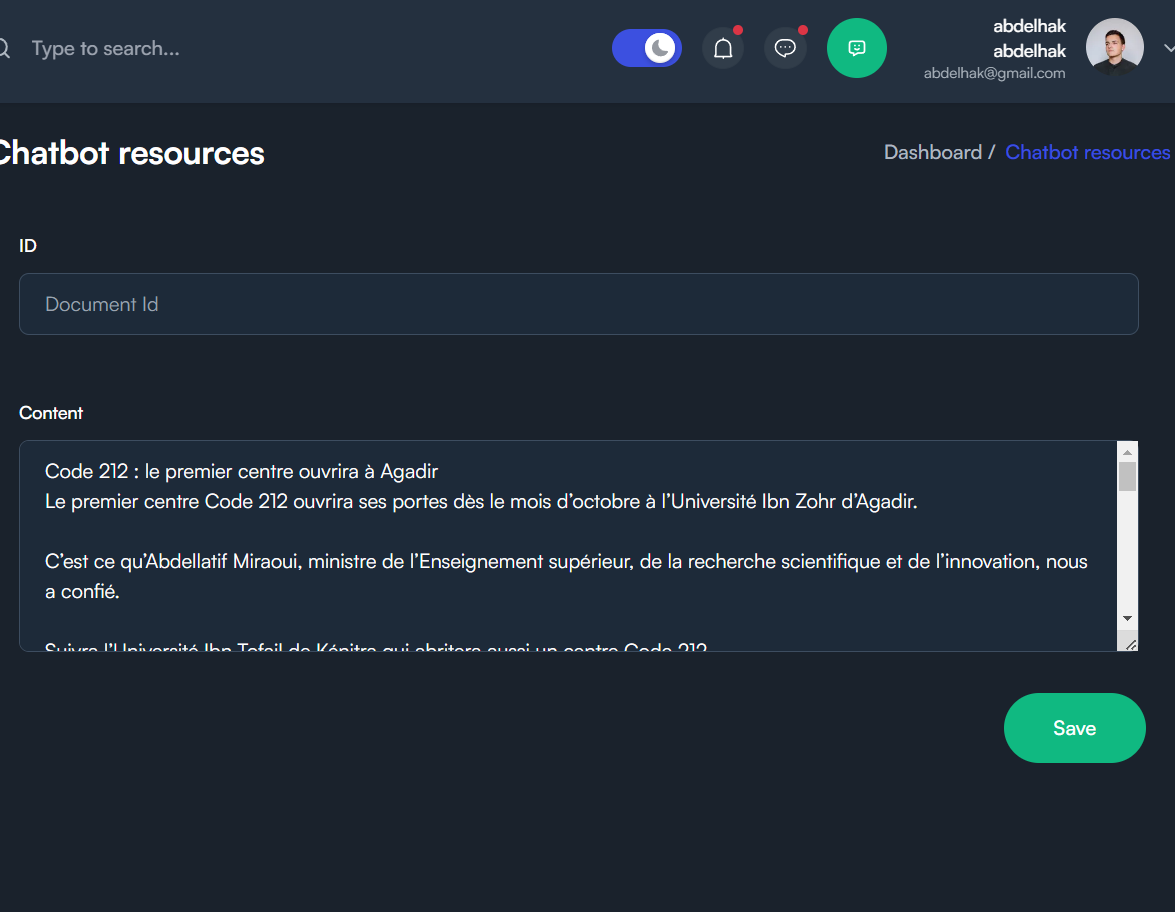
\includegraphics[height=6cm]{assets/images/admin-doc.png}
    \end{figure}
\end{frame}



\subsection{Sprint 3: Inscription aux cours, Eevenements et
    certificats}
\begin{frame}{Diagramme de cas d'utilisation}

    \begin{figure}[htpb]
        \centering
        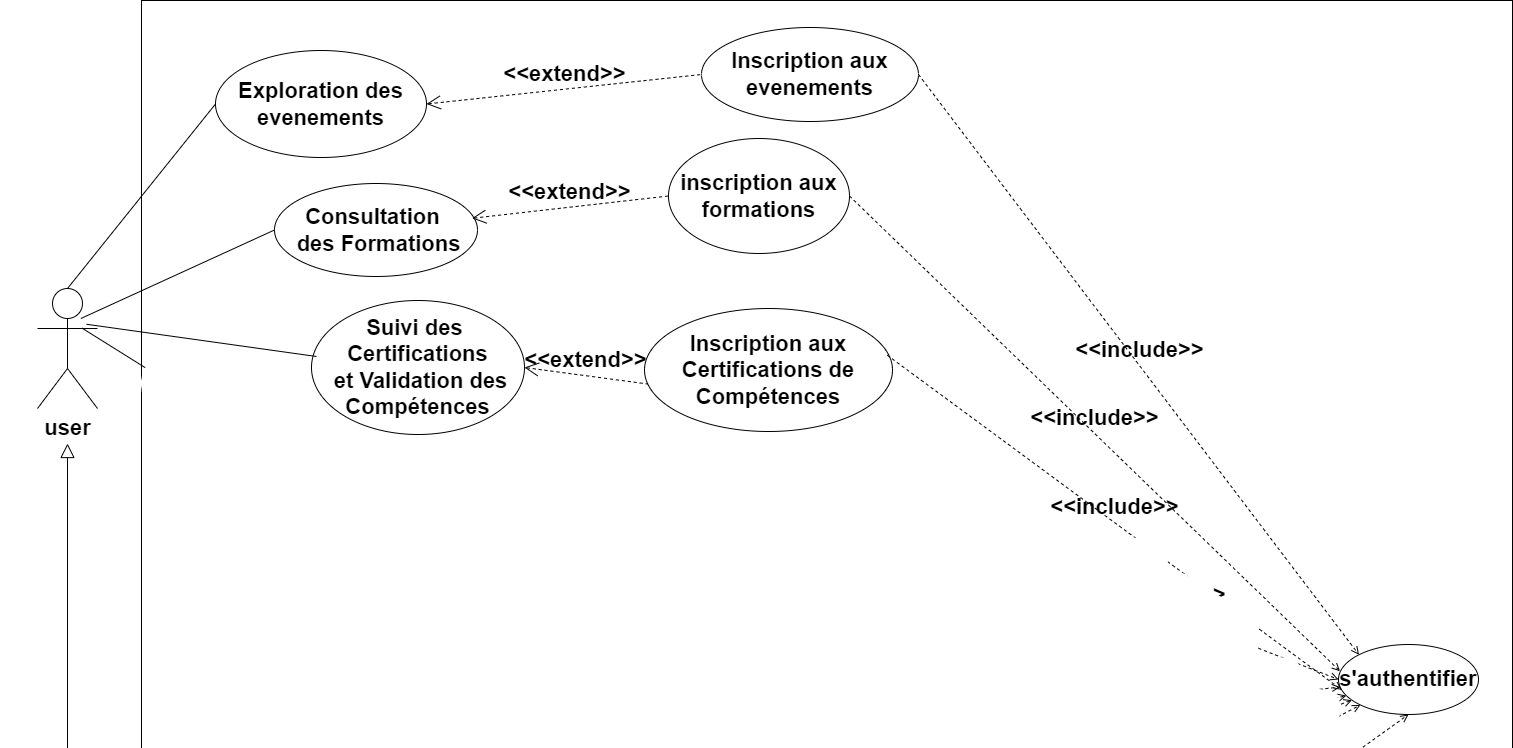
\includegraphics[height=5cm]{assets/images/sprint3-usecase.png}
    \end{figure}
\end{frame}

\begin{frame}{Diagramme de classe}

    \begin{figure}[htpb]
        \centering
        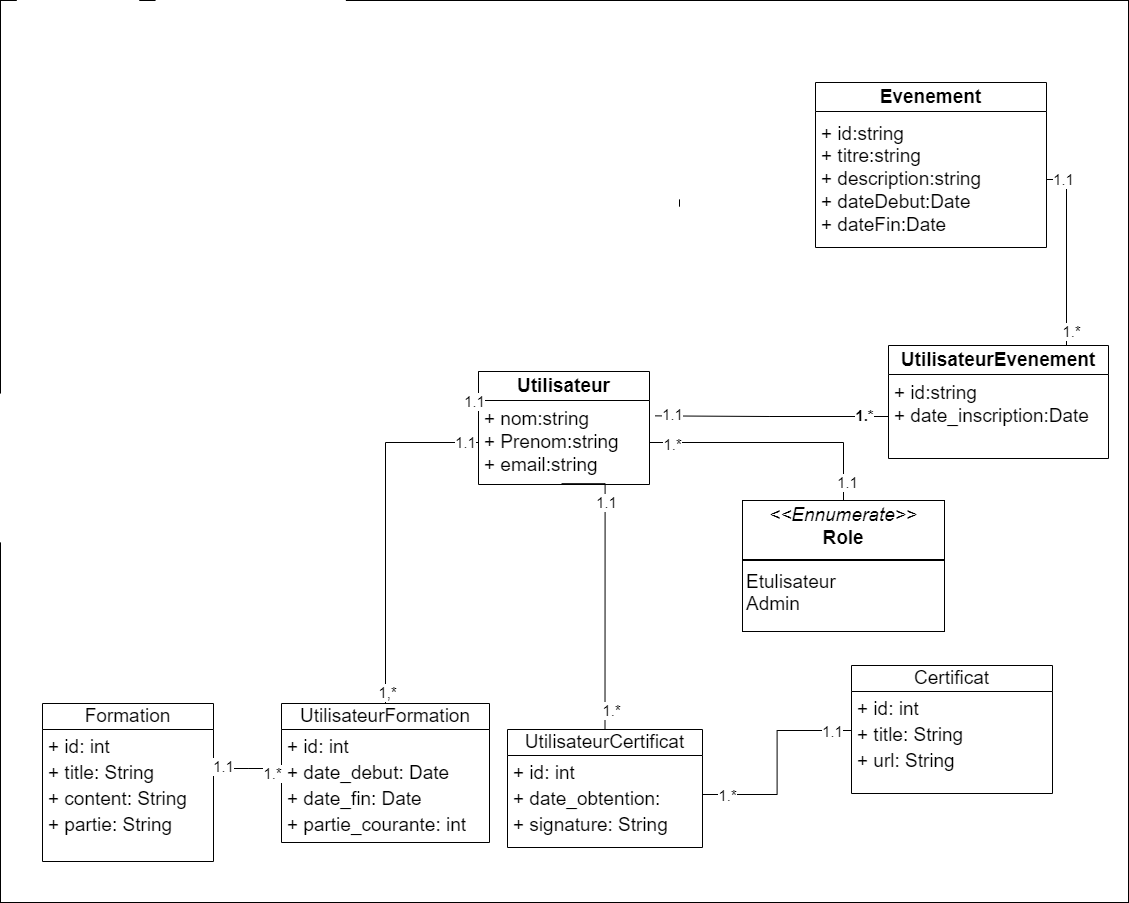
\includegraphics[height=5cm]{assets/images/sprint2-class.png}
    \end{figure}
\end{frame}


\begin{frame}{Diagramme de sequence}
    \begin{figure}[htpb]
        \centering
        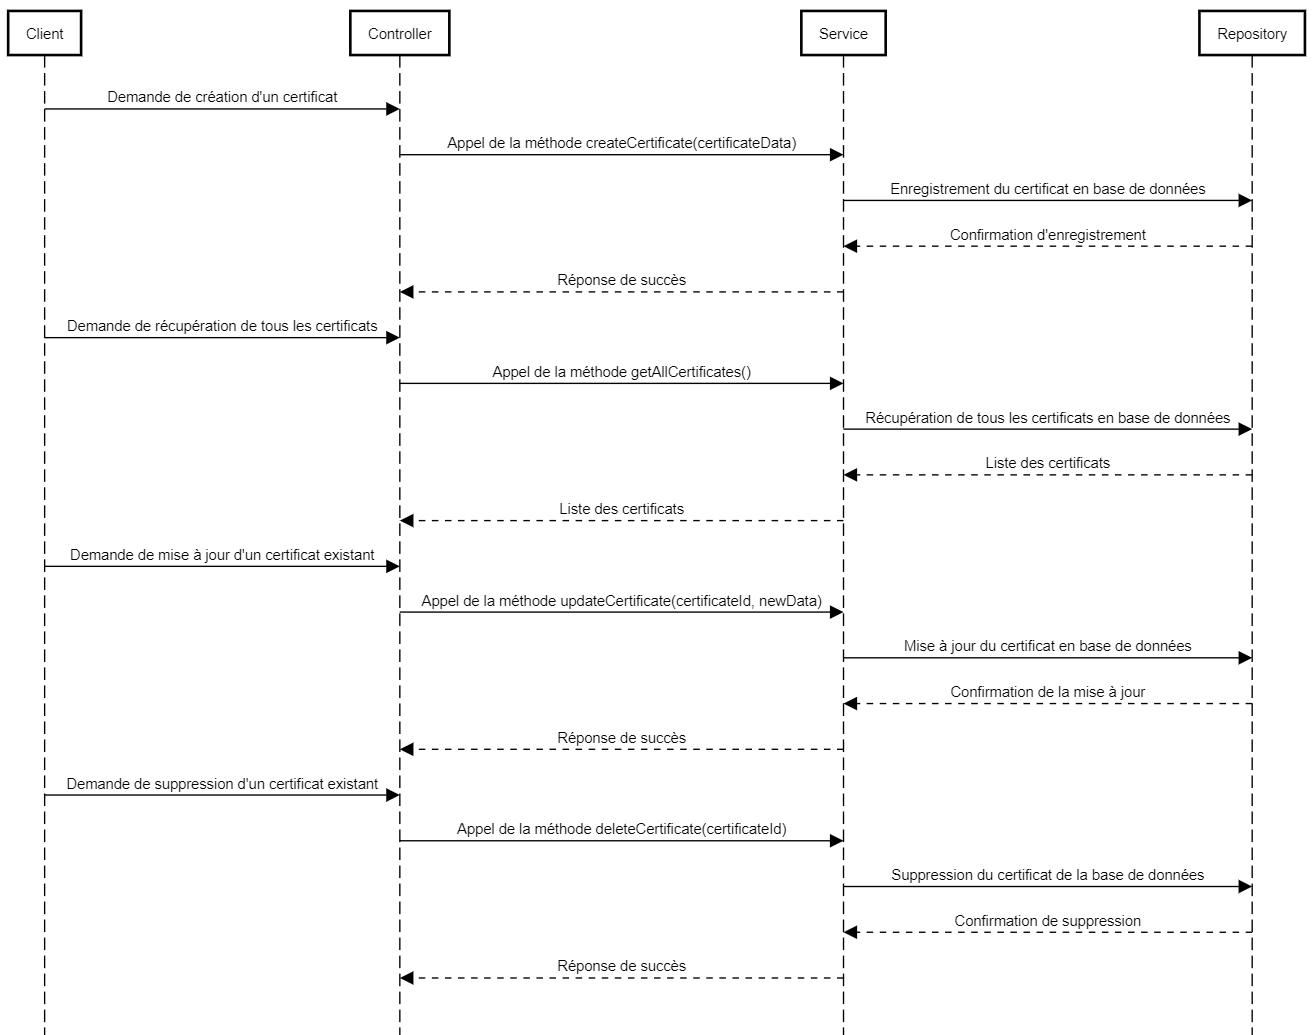
\includegraphics[height=8cm]{assets/images/seq-certifs.png}
    \end{figure}
\end{frame}

\begin{frame}{Realisation}
    \begin{figure}[htpb]
        \centering
        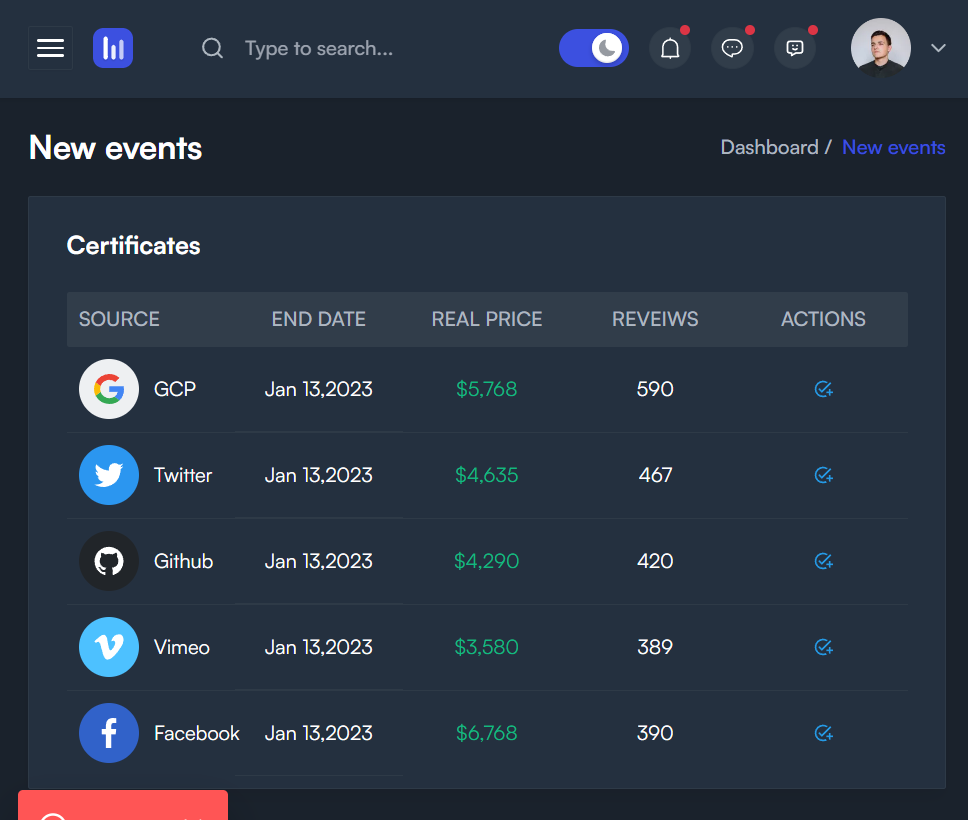
\includegraphics[height=6cm]{assets/images/certifs-list.png}
    \end{figure}
\end{frame}

\begin{frame}{Realisation}
    \begin{figure}[htpb]
        \centering
        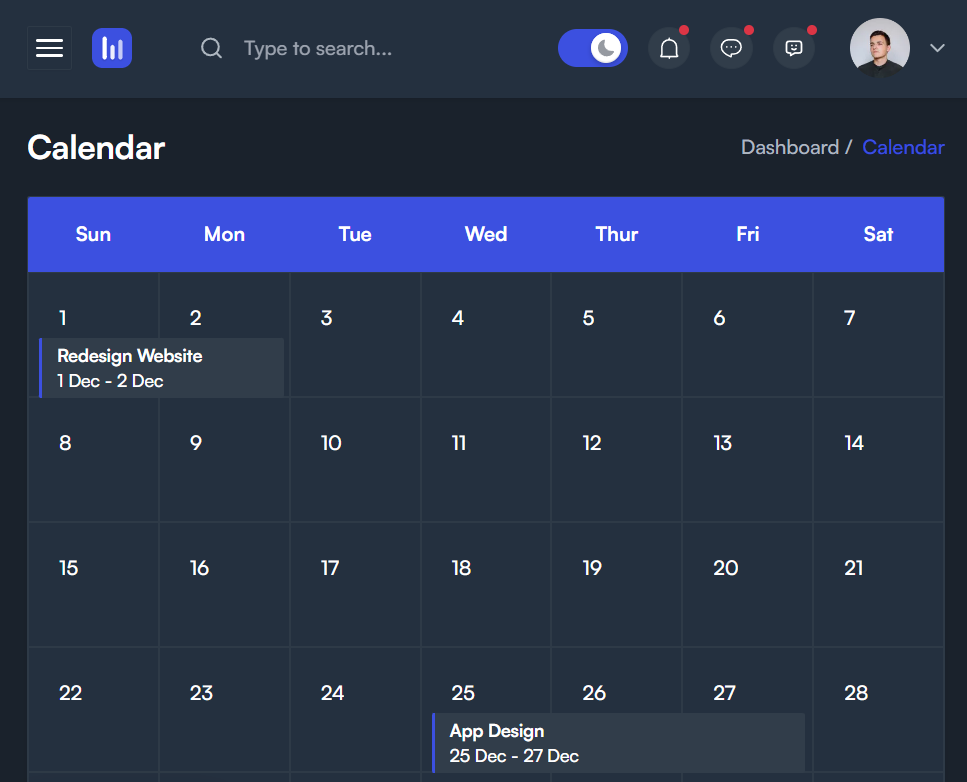
\includegraphics[height=6cm]{assets/images/calendar.png}
    \end{figure}
\end{frame}


\subsection{Sprint 4: Am´elioration de l’Interface Utilisateur et d eploiment et creation des
    contenaires}

\begin{frame}{Chat room en light mode}
    \begin{figure}[htpb]
        \centering
        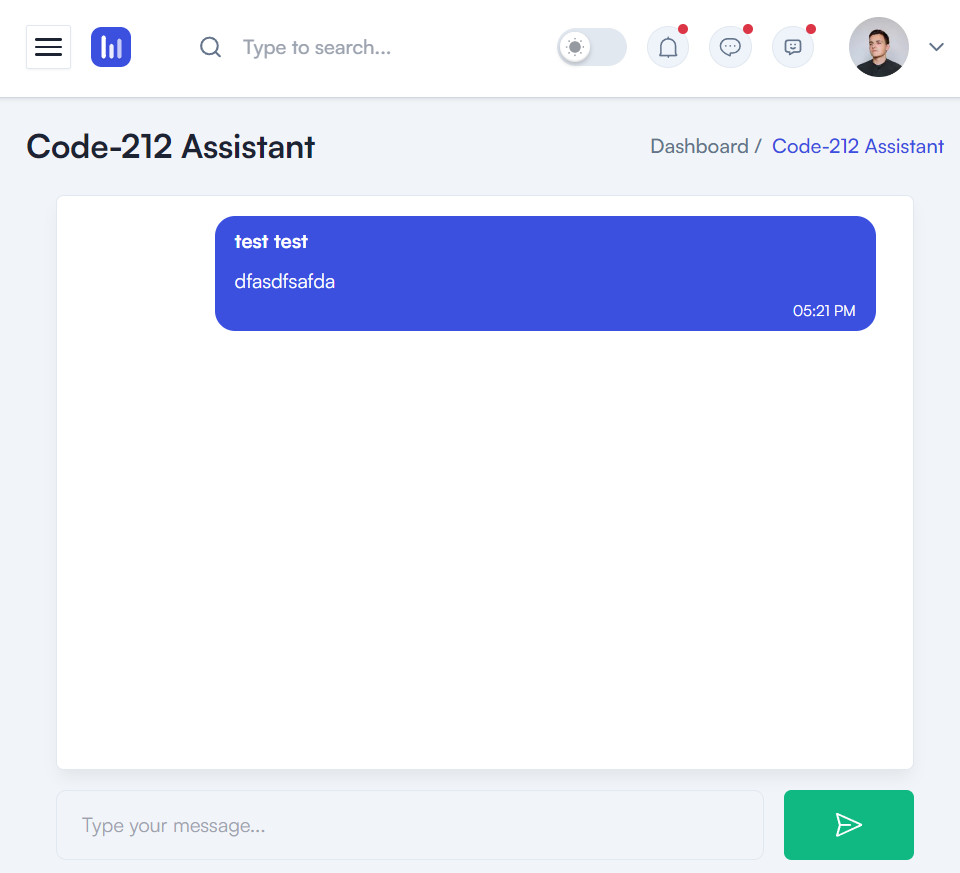
\includegraphics[height=6cm]{assets/images/light-chat.png}
    \end{figure}
\end{frame}

\begin{frame}{Profile en light mode}
    \begin{figure}[htpb]
        \centering
        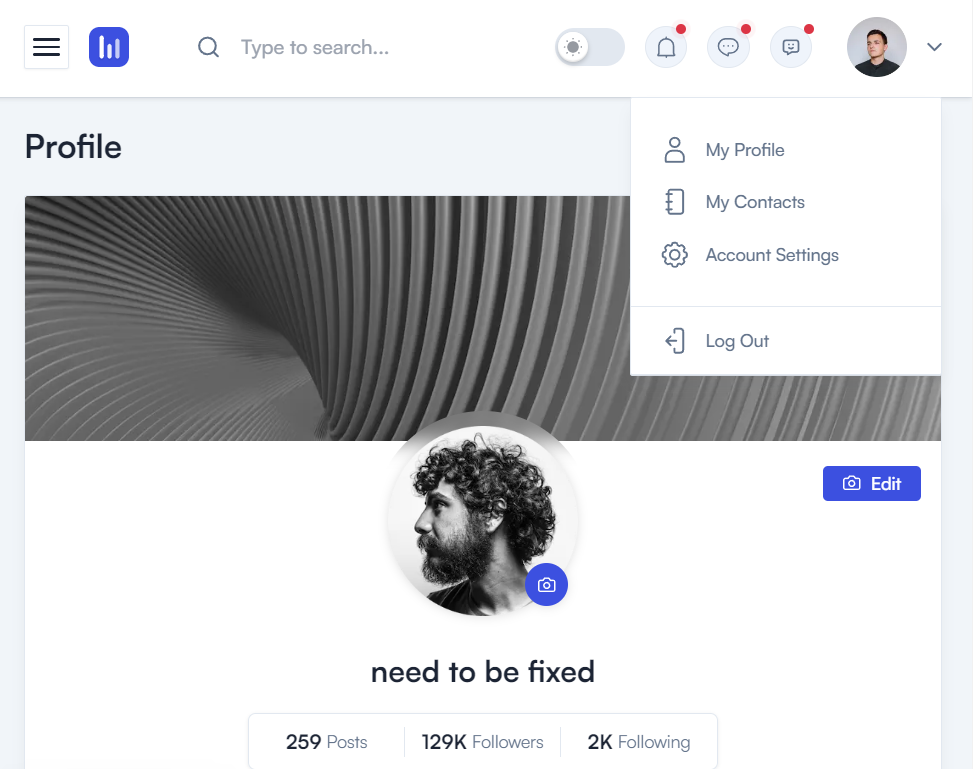
\includegraphics[height=6cm]{assets/images/light-profile.png}
    \end{figure}
\end{frame}

\subsection{Execution}
\begin{frame}{Execution}
    Demonstration de l'application
\end{frame}

\section{Conclusion}

\begin{frame}{Conclusion}
    \begin{figure}[htpb]
        \centering
        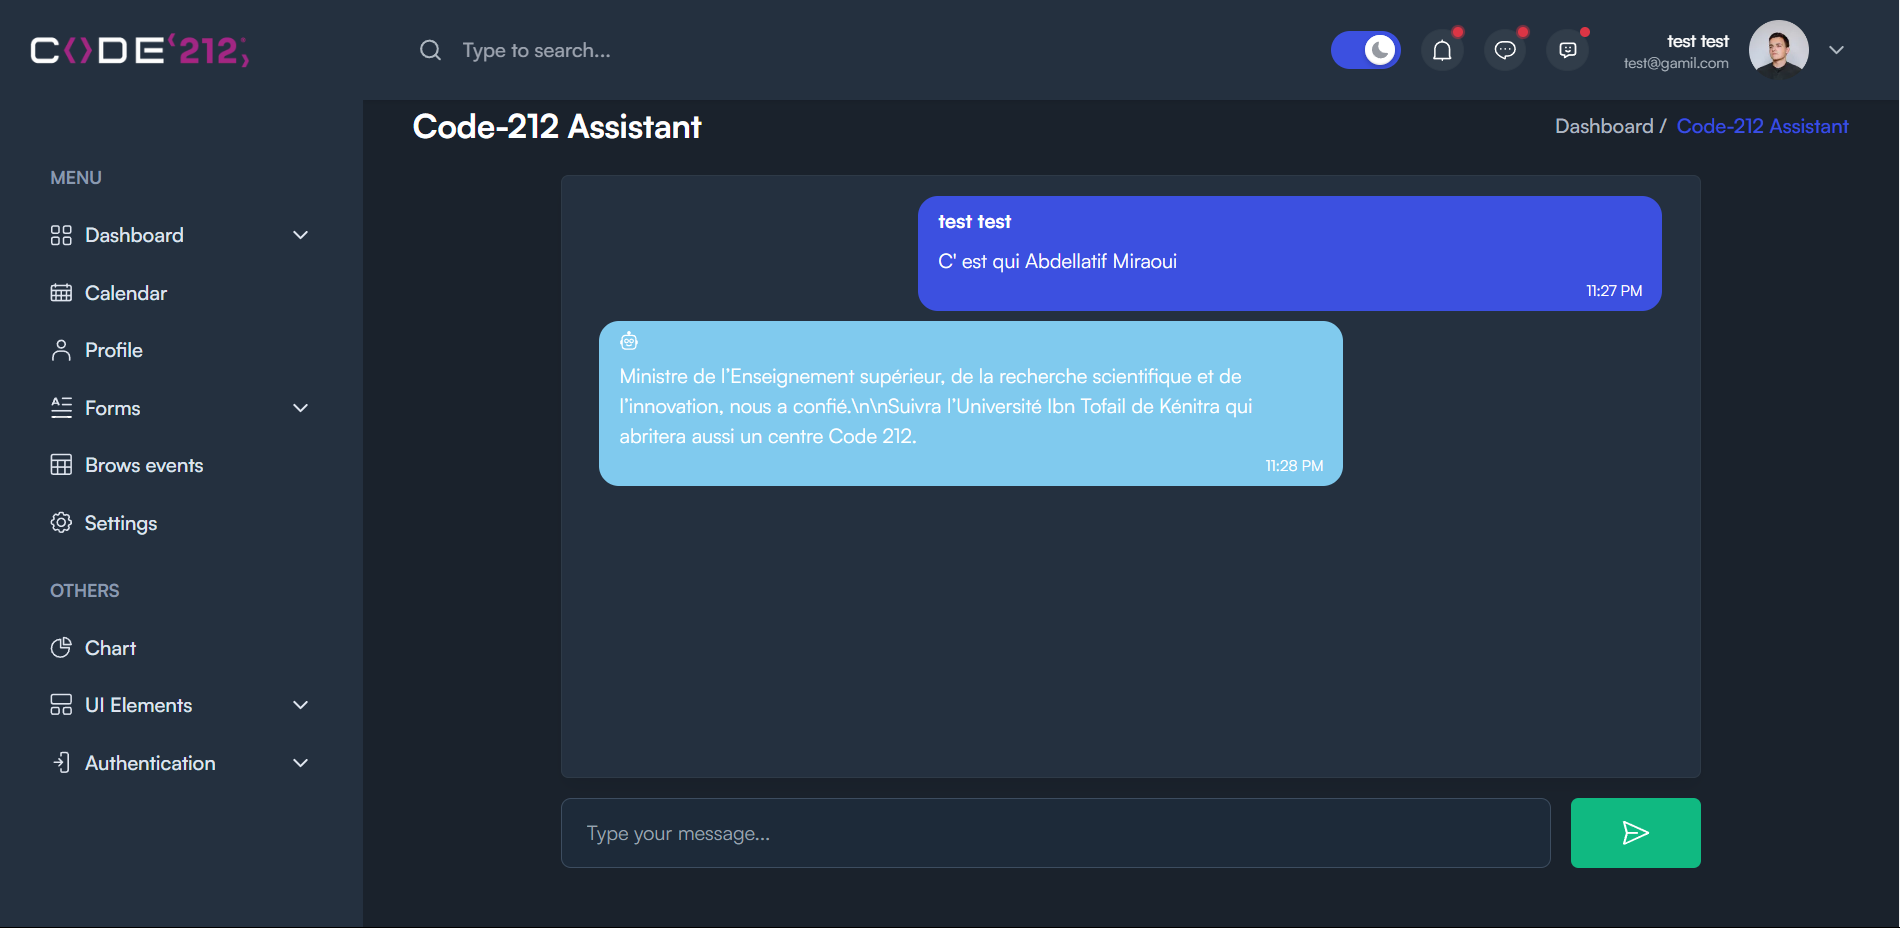
\includegraphics[height=5cm]{assets/images/chat1.png}
    \end{figure}
    En résumé, le projet vise à intégrer un chatbot AI dans une plateforme e-learning, offrant une expérience d’apprentissage améliorée pour les étudiants et une gestion efficace des cours et événements pour les gestionnaires et administrateurs.
\end{frame}


\end{document}
